
\section{Function Points: size estimation}
\subsection{Overview}



\begin{figure}[h]
	\centering
	\subfigure[FP Counting Weights]{\label{fig:fp_counting}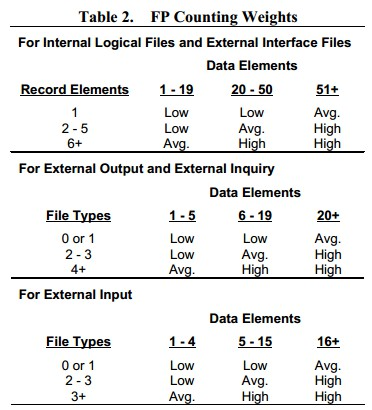
\includegraphics[width=60mm]{img/fpcounting.jpg}}
	\subfigure[UFP Complexity Weights]{\label{fig:fp_total}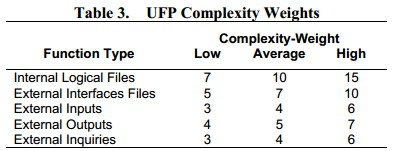
\includegraphics[width=60mm]{img/fptotal.jpg}}
	\caption{FP Analysis}
\end{figure}
\FloatBarrier


\subsection{Internal Logic Files} % (fold)

The PowerEnjoy Service needs to store information about:

\begin{itemize}
	\item \textbf{User:} This data consist in a small set of user information, for this reason its complexity has been considered \textbf{Simple}
	\item \textbf{Car:} This data consist in a small set of car information, for this reason its complexity has been considered \textbf{Simple}
	\item \textbf{Safe Area:} This data consist in a small set of safe area information, for this reason its complexity has been considered \textbf{Simple}
	\item \textbf{Trip:} This data consist in a small set of trip information, for this reason its complexity has been considered \textbf{Simple}
\end{itemize}
\fptable{			
	\fprow{User}{0}{7}	
	\fprow{Car}{0}{7}	
	\fprow{Safe Area }{0}{7}
	\fprow{Trip }{0}{7}
}{28}

\subsection{External Interfaces File} % (fold)

\begin{itemize}
	\item \textbf{GPS positioning:} This data consist on information received by user or by OnBoard device of the car. Because of the managing involve some algorithms it's considered \textbf{High}
\end{itemize}

\fptable{			
	\fprow{GPS positioning}{2}{10}	
}{10}

\subsection{External Input} % (fold)
\begin{itemize}
	\item \textbf{Sign-Up:} Create a new user in the system. The complexity has been considered \textbf{Simple}
	\item \textbf{Log-In/Log-Out:} Manage the user authentication. The complexity has been considered \textbf{Medium}
	\item \textbf{Update user information:} Update users information in the system. The complexity has been considered \textbf{Simple}
	\item \textbf{Request car reservation:} Manage the car reservation in the system. The complexity has been considered \textbf{Medium}
	\item \textbf{Unlock car:} Check if the user is nearby the reserved car and send an unlock request to the car. The complexity has been considered \textbf{Complex}
\end{itemize}

\fptable{			
\fprow{Sign-Up}{0}{3}	
\fprow{Log-In/Log-Out}{1}{4}	
\fprow{Update user information}{0}{3}	
\fprow{Request car reservation}{1}{4}	
\fprow{Unlock car}{2}{6}
}{20}

\subsection{External Inquiry} % (fold)

\subsection{External Output} % (fold)



\subsection{Results} % (fold)


